\documentclass[10pt,a4paper]{article}
\usepackage{amsmath}
\usepackage{amssymb}
\usepackage{graphicx}
\usepackage{subcaption}
\usepackage{float}
\usepackage{hyperref}
\usepackage{booktabs}

\usepackage{chato-notes}
%\usepackage[hide]{chato-notes}

\usepackage[T1]{fontenc}
\usepackage[utf8]{inputenc}

\newcommand{\abs}[1]{\left\lvert#1\right\rvert}
%\newcommand{\normnoStar}[1]{\left\lVert#1\right\rVert}

\newcommand{\spcS}{\mathcal{S}}
\newcommand{\siteS}{\mathcal{K}}
\newcommand{\condv}{\beta}
\newcommand{\spc}{i}
\newcommand{\ospc}{j}
\newcommand{\site}{k}
\newcommand{\AssMat}{A}
\newcommand{\Assv}{a}
\newcommand{\InterMat}{I}
\newcommand{\EffMat}{Q}
\newcommand{\Effv}{\alpha}
\newcommand{\ResMat}{P}
\newcommand{\Resv}{\rho}
\newcommand{\BioCont}{C}
\newcommand{\BioEff}{z}
\newcommand{\abiov}{x}
\newcommand{\abdv}{y}
\newcommand{\abioM}{X}
\newcommand{\abdM}{Y}
\newcommand{\offVect}{O}
\newcommand{\ssuit}{s}

\newcommand{\habs}{h}
\newcommand{\linkf}{f}
\newcommand{\covmap}{f}

\DeclareMathOperator{\avg}{avg}
\DeclareMathOperator{\std}{std}
\DeclareMathOperator{\dst}{d}
\DeclareMathOperator{\krnf}{k}

\newcommand{\evJoc}{$J$}
\newcommand{\evRAI}{$\Delta_{\abdv}$}
\newcommand{\evStr}{$\Effv$}

\newcommand{\trtft}[1]{\textsf{#1}}

\newcommand{\trtHeight}{\trtft{height}}
\newcommand{\trtSpread}{\trtft{spread}}
\newcommand{\trtAngle}{\trtft{angle}}
\newcommand{\trtArea}{\trtft{area}}
\newcommand{\trtThick}{\trtft{thick}}
\newcommand{\trtSla}{\trtft{sla}}
\newcommand{\trtNMass}{\trtft{nmass}}
\newcommand{\trtSeed}{\trtft{seed}}

\newcommand{\trtSlope}{\trtft{slope}}
\newcommand{\trtSnow}{\trtft{snow}}
\newcommand{\trtPhysD}{\trtft{physd}}
\newcommand{\trtZoogD}{\trtft{zoogd}}
\newcommand{\trtAspect}{\trtft{aspect}}
\newcommand{\trtForm}{\trtft{form}}

\newcommand{\sbRate}{r}
\newcommand{\hypHabs}{\phi_h}
\newcommand{\pHabs}{\theta_h}
\newcommand{\epsPos}{\epsilon^+}
\newcommand{\epsNeg}{\epsilon^-}


%%% Local Variables:
%%% mode: latex
%%% TeX-master: t
%%% End:


\graphicspath{ {./images/} }

\newcommand{\inclPlt}[2]{\includegraphics[page=#1]{tikz_figures.pdf}}
%\newcommand{\inclPlt}[2]{\input{#2}}
\usepackage{color,url,xcolor,tikz,pgfplots}
\usetikzlibrary{arrows,shapes,positioning,calc,decorations.pathreplacing,pgfplots.statistics}
\usepackage{csvsimple}
\newcommand{\datafile}{}

%%%% Grays
\definecolor{darkgrey}{gray}{0.4}
\definecolor{midgrey}{gray}{0.6}
\definecolor{lightgrey}{gray}{0.8}

%%%% Tol color scheme
\definecolor{TolDarkPurple}{HTML}{332288}
\definecolor{TolDarkBlue}{HTML}{6699CC}
\definecolor{TolLightBlue}{HTML}{88CCEE}
\definecolor{TolLightGreen}{HTML}{44AA99}
\definecolor{TolDarkGreen}{HTML}{117733}
\definecolor{TolDarkBrown}{HTML}{999933}
\definecolor{TolLightBrown}{HTML}{DDCC77}
\definecolor{TolDarkRed}{HTML}{661100}
\definecolor{TolLightRed}{HTML}{CC6677}
\definecolor{TolLightPink}{HTML}{AA4466}
\definecolor{TolDarkPink}{HTML}{882255}
\definecolor{TolLightPurple}{HTML}{AA4499}

%%%% Divergent
\definecolor{TolDivA}{HTML}{3D52A1}
\definecolor{TolDivB}{HTML}{3A89C9}
\definecolor{TolDivC}{HTML}{77B7E5}
\definecolor{TolDivD}{HTML}{B4DDF7}
\definecolor{TolDivE}{HTML}{E6F5FE}
\definecolor{TolDivF}{HTML}{FFFAD2}
\definecolor{TolDivG}{HTML}{FFE3AA}
\definecolor{TolDivH}{HTML}{F9BD7E}
\definecolor{TolDivI}{HTML}{ED875E}
\definecolor{TolDivJ}{HTML}{D24D3E}
\definecolor{TolDivK}{HTML}{AE1C3E}

%%%% Rainbow
\definecolor{TolRbwA}{HTML}{781C81}
\definecolor{TolRbwB}{HTML}{413B93}
\definecolor{TolRbwC}{HTML}{4065B1}
\definecolor{TolRbwD}{HTML}{488BC2}
\definecolor{TolRbwE}{HTML}{55A1B1}
\definecolor{TolRbwF}{HTML}{63AD99}
\definecolor{TolRbwG}{HTML}{7FB972}
\definecolor{TolRbwH}{HTML}{B5BD4C}
\definecolor{TolRbwI}{HTML}{D9AD3C}
\definecolor{TolRbwJ}{HTML}{E68E34}
\definecolor{TolRbwK}{HTML}{E6642C}
\definecolor{TolRbwL}{HTML}{D92120}

%%%% Sequential
\definecolor{TolSeqA}{HTML}{FFFFE5}
\definecolor{TolSeqB}{HTML}{FFF7BC}
\definecolor{TolSeqC}{HTML}{FEE391}
\definecolor{TolSeqD}{HTML}{FEC44F}
\definecolor{TolSeqE}{HTML}{FB9A29}
\definecolor{TolSeqF}{HTML}{EC7014}
\definecolor{TolSeqG}{HTML}{CC4C02}
\definecolor{TolSeqH}{HTML}{993404}
\definecolor{TolSeqI}{HTML}{662506}

\definecolor{colMut}{HTML}{404096}
\definecolor{colCom}{HTML}{529DB7}
\definecolor{colTro}{HTML}{7DB874} 
\definecolor{colAm}{HTML}{E39C37}
\definecolor{colCmp}{HTML}{D92120}


\tikzstyle{plate circ} = [style={draw, circle, minimum width=2.2em, minimum height=2.2em, inner sep=1, outer sep=1}]
\tikzstyle{plate sqr} = [style={draw, rectangle, minimum width=2.em, minimum height=2.em, inner sep=1, outer sep=1}]
\tikzstyle{plate arrow} = [style={->,shorten <=.5pt,shorten >=.5pt}]
\tikzstyle{pil} = [style={->,thick,shorten <=2pt,shorten >=2pt}]
\tikzstyle{net node} = [style={draw, circle, minimum width=1.8em, minimum height=1.8em, inner sep=1, outer sep=1}]
\tikzstyle{lbl node} = [style={inner sep=2, outer sep=2}]
\tikzstyle{rbl node} = [style={fill=white, inner sep=2, outer sep=2, rounded corners=2}]
\tikzstyle{tbl node} = [style={anchor=base west, align=center}] %, minimum height=1.2em}]
\tikzstyle{pnt node} = [style={fill, circle, inner sep=1}]
\tikzstyle{blg node} = [style={font=\footnotesize, anchor=south}]

%%% sparse/dense symetric/asymetric
\tikzstyle{sctSa} = [style={draw, thick, diamond, inner sep=1.5}]
\tikzstyle{sctDa} = [style={fill, diamond, inner sep=1.5, opacity=0.8}]
\tikzstyle{sctSs} = [style={draw, thick, rectangle, inner sep=2}]
\tikzstyle{sctDs} = [style={fill, rectangle, inner sep=2, opacity=0.8}]

\colorlet{cs5P}{TolDivA!40}
\colorlet{cs10P}{TolDivA!70}
\colorlet{cs20P}{TolDivA}

\colorlet{cs5N}{TolDivK!40}
\colorlet{cs10N}{TolDivK!70}
\colorlet{cs20N}{TolDivK}

% \colorlet{cs5p1}{TolDivK}
% \colorlet{cs10p1}{TolDivJ}
% \colorlet{cs20p1}{TolDivI}


\pgfplotscreateplotcyclelist{divBlue}{% 
{TolDivA, fill=TolDivA, fill opacity=0.8},
{TolDivB, fill=TolDivB, fill opacity=0.8},
{TolDivC, fill=TolDivC, fill opacity=0.8},
{TolDivD, fill=TolDivD, fill opacity=0.8}}

\pgfplotscreateplotcyclelist{divRed}{% 
{TolDivK, fill=TolDivK, fill opacity=0.8},
{TolDivJ, fill=TolDivJ, fill opacity=0.8},
{TolDivI, fill=TolDivI, fill opacity=0.8},
{TolDivH, fill=TolDivH, fill opacity=0.8}}

\pgfplotscreateplotcyclelist{divG}{%
  {darkgrey, fill=darkgrey, fill opacity=0.6},
  {darkgrey, fill=darkgrey, fill opacity=0.6},
  {darkgrey, fill=darkgrey, fill opacity=0.6},
  {darkgrey, fill=darkgrey, fill opacity=0.6}}


\pgfplotsset{
	compat=1.8,
	clip = false,
	clip marker paths = true,
	tick align=outside,
    tick align=inside,
    xtick pos=left,
    ytick pos=left,
	x tick label style = {yshift=-1em, anchor=base},
	major tick length = 2pt,
    %every axis y label/.style = {at = {(ticklabel cs:0.5)}, rotate=90, anchor=center, font=\scriptsize, xshift = -2pt},
	%every axis x label/.style = {at = {(ticklabel cs:0.5)}, anchor=base center, font=\scriptsize, yshift = -2pt},
%	axis y line*=left, axis x line*=bottom,
}

%%% Local Variables:
%%% mode: latex
%%% TeX-master: "modelE"
%%% End:


%opening
\title{Uncovering ecological associations by learning latent representations of species effects and responses from their co-distribution}
\author{Sara Si-moussi, Esther Galbrun, Mickael Hedde, Wilfried Thuiller}

\graphicspath{ {./images/} }
\begin{document}

\maketitle

\section{Background}
Understanding the drivers of species distribution and their abundance has always been a long-lasting goal of biogeography \cite{humboldt1805essai}. Niche theory explains the spatial dynamics of species by a set of physiological and adaptive properties that lead them to thrive in specific conditions and decline in others (\cite{chase2003ecological}, \cite{pulliam2000relationship}). The ranges of abiotic variables, such as climate and soil characteristics, that match the ecophysiological requirements of a species delimit its potential niche (Grinnellian niche, \cite{grinnell1917niche}) or (Fundamental niche, \cite{hutchinson1957multivariate}).  Habitat suitability models (HSM) or species distribution models (SDMs) \cite{guisan2017habitat} aim to infer and model this niche by establishing statistical relationships between observed occurrences or abundances of species and the environmental characteristics of the corresponding locations. \\

HSMs have proven useful to predict species ranges in response to climate change, providing operational tools to conservation biologists (\cite{guisan2005predicting}, \cite{elith2009species}). However, as they model multiple species distributions separately, they fail to detect possible dependencies between species that can restrict or extend their ranges beyond what is expected when considering only abiotic factors.  Indeed, species may exclude one another locally (\textit{competitive exclusion}, \cite{hardin1960competitive}) or differentiate each other’s areas and resources (\textit{niche partitioning}, \cite{schoener1974resource}). Conversely, some species facilitate others by modifying the environment in a way that creates habitats or enables access to resources for other species (engineering and facilitation). Although these interactions take place at a local scale, some of them may alter the range of the species on a wider, macroscopic scale. Consequently, they induce consistent patterns of colocation and dislocation that are unexplained by the abiotic environment, referred to as \emph{associations}. The inability to take into account the presence or absence of other species is therefore an important source of underfitting for statistical models of species distributions (\cite{wisz2013role}). \\

Over the last decade, several approaches have been proposed to infer interspecific dependencies from the observations of many species. Probabilistic Graphical Models (PGM) \cite{koller2009probabilistic} have been used to infer either directed (Bayesian Networks, BN) or undirected (Markov Random Fields, MRF) networks \cite{faisal2010inferring} involving plants \cite{aderhold2012hierarchical}, parasites and potential hosts \cite{pilosof2014host}, predators and preys \cite{trifonova2015spatio}\cite{majdi2018there} or multi-trophic communities turnover \cite{ohlmann2018mapping}. More recently, Joint Species Distribution Models, JSDM (\cite{pollock2014understanding},\cite{ovaskainen2017make}) attempted to address the same question while jointly predicting co-occurrences of multiple species. Their gist is that once we have accounted for abiotic factors, the unexplained variance, typically captured by the residuals' correlation matrix, is attributed to the effect of species on one another.  As they rely purely on correlation, JSDMs and MRFs are limited to estimating symmetric associations where the involved parties influence one another with the same polarity and strength. \cite{lany2018asymmetric} proposed a JSDM that allows to capture asymmetric associations but it requires access to longitudinal data. On the other hand, BNs support directed relationships but they impose an acyclic structure that hinders the modeling of bidirectional influences. \\

Another research domain that is also concerned with inferring associations from co-occurrence is natural language processing (NLP). NLP modelers try to understand semantic associations between words on the basis of the contexts they appear in. The context of a word is the list of words surrounding it in a sentence. A state of art method in this area is \texttt{word2vec} (\cite{mikolov2013distributed}). \texttt{word2vec}  learns distributed representations for words in the form of dense vectors called embeddings. The embedding of a word captures information about other words it co-occurs with. The probability of a word occurring in a particular sentence of a text depends on the semantic compatibility of this word with other words occurring in that sentence. Word embeddings, such as \texttt{word2vec} , aim to learn multidimensional representations of words that captures this contextual semantic compatibility. By analogy, in community ecology, the probability of the presence of a species in a given abiotically suitable site depends on its compatibility with other species occuring at that site, i.e. other species in the observed community. \\

\cite{rudolph2016exponential, liu2017zero} introduced a generalization of word embeddings to any type of data that follow an exponential family distribution, including binary and ordinal data, called exponential family embeddings. Building on existing work, we propose a conditional probabilistic model of species co-distributions that can be trained jointly with any habitat suitability model on presence/absence or count data to infer interspecific associations. We evaluate the potential of the model to recover correct associations on empirically observed as well as simulated communities.

\section{Material and Methods}
Three main conditions should be satisfied for a species to inhabit a given location. First, the location must be accessible. This relates to the intrinsic dispersal capacity of the species and the presence of migration opportunities or barriers.  Second, the abiotic conditions should allow the species' population to maintain a positive growth rate. This condition is referred to as \emph{habitat suitability} and is the target of Habitat Suitability Models. Third, intraspecific and interspecific interactions within communities can also alter the range of the species as well as their local abundances (\cite{guisan2017habitat}). Although we recognize the importance of spatial dispersal processes, in this study we focus on the latter two factors, namely \emph{habitat suitability} and \emph{species interactions}, also refered to as the \emph{abiotic} and \emph{biotic} factors, respectively.\\

We consider a dataset consisting of the abundances of a collection $\spcS$ of $m$ species observed at a collection $\siteS$ of $n$ sites, as well as environmental variables measured at these same sites or in their vicinity.The abundance of species $\spc$ at site $\site$ is noted $\abdv_{\site\spc}$. The abiotic environment in site $\site$ is represented by the \emph{abiotic feature} vector $\abiov_{\site}$ computed by applying a feature extraction model on the raw environmental variables. \\

In what follows, we introduce key concepts used in the inference model. In particular, we explain how we model the interactions between a pair of species by decomposing them into effects and responses represented as multi-dimensional embedding vectors and how we use these embeddings to represent the biotic factors.

\subsection{Biogeographical associations and biotic context}
A \textit{biogeographical association} describes the relative influence of a pair of species on one another's abundances.  The two directions of this influence can be of different types (positive, negative or neutral) and have different intensities.  An association represents a consistent pattern of co-occurrence with potentially multiple mechanistic explanations: a direct biotic interaction, an indirect interaction through the environment or a shared correlation to an unmeasured environmental variable or an unobserved group of organisms.

\subsubsection{Representing species associations using embeddings}
Formally, we represent the association between species $\spc$ and
$\ospc$ with a pair of numerical values $\Assv_{\spc\ospc}$ and
$\Assv_{\ospc\spc}$, representing the strength of the influence of species
$\ospc$ on species $\spc$ and vice-versa, respectively. Specifically,
$\Assv_{\spc\ospc}$ represents the change (excess if
positive, deficit if negative, none if null) in \textit{target}
species $\spc$'s abundance induced by the presence of an individual
from \textit{source} species $\ospc$.  These values across all pairs of
species can be collected into an $m \times m$ non-symetric association
matrix $\AssMat$. \\

\begin{figure}[bthp]
	\centering
	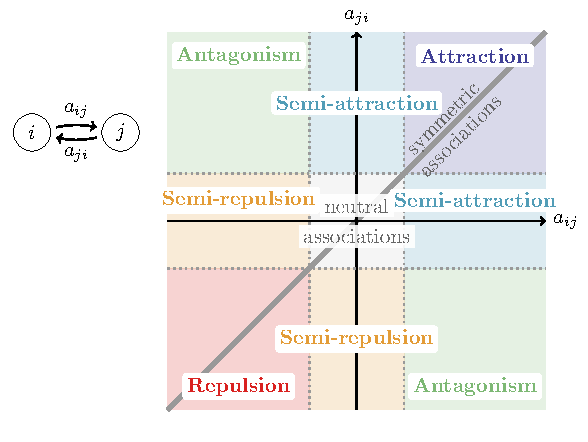
\includegraphics[page=1]{tikz_figures.pdf}
	\caption{Mapping pairwise association strengths to potential interaction classes. The first bissector represents the association domain covered by correlation-based approaches and undirected graphical models.}
	\label{assocdomain}
\end{figure}

The association strength depends on two latent parameters: the \textit{effect} applied by the source and the \textit{response} of the target. We assume these parameters are controlled by intrinsic traits of the species, which we encode in two separate $d$-dimensional real-valued vectors referred to as embeddings.
In practice, $d$ is a user defined parameter which is typically significantly smaller than half the number of species. \\

The \emph{effect embedding} of species $\spc$ is denoted as $\Resv_\spc$, it captures the type of organisms the species allows when it is present. The \emph{response embedding} of species $\spc$ is denoted as $\Effv_\spc$, it controls the type of biotic context the species would strive in. For instance, trees with spreading canopy create shade (effect) that selects only shade-tolerant (response) species and exclude others. The response and effect embeddings of the different species can be collected into two $m\times d$ matices, respectively denoted as $\ResMat$ and $\EffMat$. \\

The association matrix is then written as
\begin{equation*}
	\AssMat = \ResMat\EffMat^{T}
\end{equation*}

\begin{figure}[bthp]
  \centering
  \includegraphics[page=2]{tikz_figures.pdf}
  \caption{Association matrix factorization.}
  \label{factoriz}
\end{figure}

\subsubsection{Biotic context}
The biotic context encodes our assumptions about potential biotic effects a target species is exposed to in a given site. In the simplest case, without any prior knowledge, it is formed of individuals from other species observed in the same location. Specifically, the biotic context of species $\spc$ in site $\site$, denoted $\BioCont_{\site\spc}$, is computed as follow:
\begin{equation*}
\BioCont_{\site\spc} = \{\ospc \in \spcS, \ospc \neq \spc ~\text{and}~ \abdv_{\site\spc} > 0 \}
\end{equation*}

We obtain the aggregated effect of the biotic context by averaging the effect embeddings of its elements weighted by their respective abundances:   
\begin{equation*}
\BioEff_{\site\spc} = \frac{1}{\abs{\BioCont_{\site\spc}}} \sum_{\ospc \in \BioCont_{\site\spc}} \abdv_{\site\ospc} \Effv_{\ospc}
\end{equation*}

This formulation allows the compensation between the presence of facilitators and competitors. By weighting with abundance, we consider implicitely that individuals from the same species are similar and contribute equally to the community structure. Conversely, the effect of rare species would only be apparent if their per capita effect is stronger than the aggregated effect of dominant groups.\\

The biotic context carries implicit constraints on the structure of species association networks by restricting the set of potential associations a priori. We present some alternative definitions of the biotic context with the associated data requirements and relevant effect aggregation functions in the appendix (see Section~\ref{sec:alt-bio}). 

\subsection{A conditional generative model of abundance}

\subsubsection{Formalization}
The indicator of abiotic suitability for species $\spc$ at site $\site$, denoted $\ssuit_{\site\spc}$, follows a Bernoulli distribution, whose parameter (success rate) is given by a habitat suitability model (HSM), $\habs$, fitted on the target species's occurrences.
\begin{equation*}
    \ssuit_{\site\spc} \sim \mathcal{B}(\habs_{\spc}(\abiov_{\site}))
\end{equation*}

\begin{figure}[bthp]
  \centering
  \begin{minipage}{0.58\textwidth}
    \includegraphics[page=3]{tikz_figures.pdf}
    \end{minipage}
    \begin{minipage}{0.33\textwidth}
    \begin{tabular}{ll}
      \toprule
    $d$ & embedding dimension \\
    $\abiov$ & abiotic feature vector \\
    $\ssuit$ & abiotic suitability \\
    $\BioCont$ & biotic context \\
    $\Resv$ & species response \\
    $\Effv$ & species effect \\
    $\abdv$ & species abundance \\
    $\BioEff$ & biotic context effect \\
    \bottomrule
    \end{tabular}
  \end{minipage}
  \caption{Plate diagram of the generative model of abundance.}
  \label{plate}
\end{figure}

At sites where the abiotic environment is not suitable (i.e.\ where $\ssuit_{\site\spc} = 0$), the probability mass of the species abundance is concentrated on zero. In other words, $\eta_{\site\spc}$ follows the Dirac delta function denoted as $\delta_0$. Otherwise (i.e.\ where $\ssuit_{\site\spc} = 1$), the abundance of the species is a function of its biotic context. \\

Following (Rudolph et al.\ 2016), we model the abundance using the canonical form of the exponential family $\mathcal{E}$ parameterized by $\eta_{\site\spc}$.
\begin{equation*}
\abdv_{\site\spc} \sim \left\{
\begin{array}{ll}
\mathcal{E}(\eta_{\site\spc},\tau_{\site\spc}) & \mbox{if } \ssuit_{\site\spc}=1, \\
\delta_0 & \mbox{otherwise.}\\
\end{array}
\right. \\
\end{equation*} \\

We let the canonical parameter $\eta_{\site\spc}$ depend on the response $\Resv_\spc$ of the target species and the biotic context effect $\BioEff_{\site\spc}$. An offset $o_{\spc}$ is used to represent the baseline abundance for each species in the event of an empty biotic context. Link function $\linkf$ scales the outcome to the domain of the target variable. 
%When the offset is set to zero, the target species would need a facilitator to be present. %

\begin{equation*}
  \eta_{\site\spc} = \linkf(\Resv_\spc \BioEff_{\site\spc} + o_\spc)
\end{equation*}
which can be rewriten as an aggregate of pairwise association strengths:

\begin{equation*}
  \eta_{\site\spc} = \linkf\big( \sum_{\ospc \in \BioCont_{\site\spc}} \abdv_{\site\ospc}  \Assv_{\spc\ospc} + o_\spc\big) \\
\end{equation*} 

%When the offset is set to zero, the target taxa would need a facilitator to be present. %

Different choices of probability distributions, depending in particular on the type of data considered (presence/absence vs. abundance) result in different instanciations of this generic model.
In Table \ref{paramap}, we provide the mapping from the natural parameter to the expression of the mean for different choices of the link function in the special cases where $\mathcal{E}$ is a binomial (with fixed number of trials), a negative binomial (with fixed number of failures) or a Poisson distribution. 

\begin{table}[bthp]
  \centering
  \begin{tabular}{llll}
    \toprule
	Data type & Distribution & Link function & Natural parameter mapping \\ 
    \midrule
	Presence/Absence & Binomial  & identity  & Probability of occurrence \\ 
	 & & & $p_{\site\ospc}=\sigma(\sum_{\spc \in \BioCont_{\site\spc}} \abdv_{\site\ospc}  \Assv_{\spc\ospc} + o_\spc\big)$ \\
	 & & & $\sigma$ : logistic function \\
	 
	 \midrule
	
	Count & Poisson  & identity  &  Mean count \\
	& & & $\lambda_{\site\spc}=\exp(\sum_{\ospc \in \BioCont_{\site\spc}} \abdv_{\site\ospc}  \Assv_{\spc\ospc} + o_\spc\big)$ \\
	
	\midrule
	
	Count & Poisson  & logarithm  &  Mean count \\	
	& & & $\lambda_{\site\spc}=(\sum_{\ospc \in \BioCont_{\site\spc}} \abdv_{\site\ospc}  \Assv_{\spc\ospc} + o_\spc\big)$ \\
	
	\midrule
	
	Count & Negative binomial  & identity  &  Mean count \\
	& & & $p_{\site\spc}=\exp(\sum_{\ospc \in \BioCont_{\site\spc}} \abdv_{\site\ospc}  \Assv_{\spc\ospc} + o_\spc\big)$ \\
	
    
    \bottomrule
\end{tabular}
\caption{Natural parameter mapping and link function choices for common distributions used for presence/absence or count data.}
\label{paramap}
\end{table}

\subsubsection{Inference}
Having formalized our model, we now outline the inference process, i.e.\ the procedure for training the model. \\

In order to prepare the examples for training the model, we gather as positive and negative examples respectively the species that are present and absent at each site $\site$:
\begin{align*}
\mathcal{S}_{\site}^+ &= \{\spc \in \spcS, \abdv_{\site\spc}>0\} \\ 
\mathcal{S}_{\site}^- &= \{\spc \in \spcS, \abdv_{\site\spc}=0\}
\end{align*}

Negative examples are typically overrepresented in the dataset, leading to a high inbalance between positive and negative examples. Therefore, we sub-sample negative examples, selecting $\sbRate \%$ of them at random into the training set, alongside all positive examples. By introducing noisiness into the objective function, this sub-sampling procedure also improves the robustness of the estimations and prevents overfitting. Furthermore, we promote the sparsity of the embeddings and of the resulting association matrices by adding lasso penalties on the embedding vectors. \\

Our model is then trained on this collection of labelled examples. Specifically, we maximize the likelihood of the observed abundances on each site for all positive examples and the selected subset of negative examples. \\

In summary, given training data (abundances $\abdM$ and abiotic variables $\abioM$) together with user-defined hyperparameters (including hyperparameters for the abiotic suitability model $\hypHabs$, embedding dimension $\dst$, vector of species offsets $\offVect$, negative examples subsample rate $\sbRate$ and regularization coefficient on the constraint of embeddings sparsity $\lambda$) the model training procedure aims to infer the value of the model parameters (esp.\ the response and effect embeddings matrices $\ResMat$ and $\EffMat$, and the HSM parameters $\pHabs$) that optimize the objective function. 

To do so, we use online stochastic gradient descent with a scheduled learning rate decay and a glorot uniform initializer for the parameters.\\

%%% Temporary %%%
The resulting model can then be applied on previously unseen data, e.g.\ environment features for sites not included in the training data, to predict abundances at these sites for each of the species in the training data given the abundances of other species.
%%% %%%%

\subsection{Unraveling inter-specific association networks}
While the primary task addressed by our model is the prediction of abundances, the effect and responses embeddings are also learnt, as by-products of the inference. In fact, these embeddings for the different species, contained in matrices $\EffMat$ and $\ResMat$, as well as the resulting non-symmetric association matrix $\AssMat$ are of great interest, as they shed light on the ecological association between the species. \\

In order to identify meaningful associations, we apply two filtering steps to the matrix $\AssMat$ returned by our model. First, the \emph{statistical filtering} step consists in setting to zero all associations with a confidence interval containing zero and keeping the mean value for the rest. Second, the \emph{biogeographical filtering} step aims to further eliminate associations that are predicted to potentially exist from the latent representations of the species, but are not realized by the species occurrences because they break some biogeographical constraints. \\

For instance, mutualism or attraction between two species requires co-existence. Thus, we set to zero any inferred positive effect involving two non-co-occurring species (\cite{sanderson2015patterns}). On the other hand, repulsive relationships do not require co-occurrence and may even explain the geographic separation. Hence, the involved species do not have to co-occur but should live in similar environments for us to consider a potential negative association to be valid. Specifically, we compute the ranges of the environmental values corresponding to the occurrences of either species and retain negative associations only if these ranges overlap or if the species are otherwise sufficiently similar (above a user-defined similarity threshold) in terms of their habitat suitability parameters, which capture the species' respective habitat preferences. \\

Furthermore, we are often more interested in the polarity of the associations, rather than their precise strength, hence we consider a discretized version of the association matrix, which we call the \emph{adjacency matrix} defined as follows:
\begin{equation*}
\InterMat_{\spc\ospc} =  \left\{
\begin{array}{ll}
\text{positive} & \mbox{if } \AssMat_{\spc\ospc}>\epsPos, \\
\text{negative} & \mbox{if } \AssMat_{\spc\ospc}<\epsNeg, \\
\text{neutral} & \mbox{otherwise.}
\end{array}
\right.
\end{equation*}

such that $\epsPos$ and $\epsNeg$ represent a user-defined threshold on the strength of the positive and negative associations, respectively. \\

The adjacency matrix describes a network, where each species is represented by a vertex and a directed edge labelled as positive (resp.\ negative) from vertex $\spc$ to vertex $\ospc$ represents a positive (resp.\ negative) influence of species $\spc$ on species $\ospc$. In this context, inferring associations can be seen as an edge prediction task, i.e.\ the task of predicting the existence and polarity of an edge for any ordered pair of species.\\

Assuming that the ground-truth network is available (in the form of the simulation parameters in the case of simulated populations, for instance), we can evaluate the performance of our model on this prediction task by comparing the network constructed from inferred parameters in matrix $\AssMat$ to the ground-truth using standard multi-class classification performance metrics (recall, precision, F1-score).\\

Note that species with similar response embeddings constitute clusters of rows in the adjacency matrix, called \emph{response groups}. Conversely, species with similar effect embeddings constitute clusters of columns called \textit{effect groups}. The product of both types of groups, results in the emergence of clusters of exchangeable or redundant species occupying the same \emph{structural roles} in the resulting network \cite{gauzens2015trophic}. 

\subsection{Validation on simulated data}
Before applying our proposed model on real-world datasets, we perform a validation experiment in a controlled setting. That is, we evaluate the ability of our model to recover interspecific associations from simulated datasets of known associations.\\

\subsubsection{Data Generation}
We use a process-based stochastic model adapted from \texttt{Virtualcomm} (Gallien and Münkemüller 2015) to simulate the assembly of individuals from a regional species pool into communities, on different locations sampled along an environmental gradient. The assembly process is controlled by three filtering mechanisms: the response to the abiotic environment, the outcome of biotic interactions and reproduction.  For simplicity, the spatial structure of communities and thus dispersal processes are ignored. In other words, there is no exchange of individuals between neighboring communities.\\

The simulation starts with a given or random initial composition for each community independently. Individuals are replaced through time until an equilibrium state is reached or a user-defined number of iterations is completed. In the end, the final composition of the communities is returned as the result of the simulation.\\

We set up an experiment similar to (Pollock et al, in prep) where multiple simulations are run on random points on a gradient between 0 and 100 with different hand-crafted configurations of the prior interaction matrix. Specifically, four configuration modes were tested: absence of association, positive associations only, negative associations only and both positive and negative associations. In each mode, we vary the number of species (5, 10 or 20), the proportion of associated pairs (sparse or dense) and whether the association matrix includes asymmetric effects. Positive (resp.\ negative) effects were all set to $+1$ (resp.\ minus $-1$) as we are interested in the polarity of the associations rather than their magnitude. The full-factorial design of this experiment produced 29 simulation datasets, summarized in Figure \ref{simexp}).\\

\begin{figure}[bthp]
  \centering
  \includegraphics[page=4]{tikz_figures.pdf}
  \caption{Design of the simulation experiment.}
  \label{simexp}
\end{figure}

\subsubsection{Model training}
For each simulated population dataset, we count the number of individuals of each species in each site to produce a site-by-species abundance matrix and binarize these counts to produce a site-by-species occurrence matrix. 
As our HSM models for the abiotic response of the species, we use independent Generalized Linear Models (GLM) with logistic links and one quadratic term.\\

We apply the proposed association inference model with a negative binomial distribution to fit the species counts. We set the offsets for each species as the average value of its abundance on its sites of presence (i.e.\ $o_\spc=\bar{\abdv}_{\spc}$). We also add lasso penalties with $\lambda=0.01$ on response and effect embeddings to promote the sparsity of their products. \\

To adjust the embeddings dimension $d$, we use a $5$-fold cross-validation scheme where we monitor the deviance of the predicted abundances. Having set $d$ to the value that minimizes the deviance, we train the model on $1000$ bootstrap samples from the training set. \\

Given the observed count $y$ and the predicted mean count $\mu$, the deviance is computed as two times the difference between the predicted and the maximum achievable likelihoods. The latter is simply the likelihood on the observed count value.  

\begin{equation*}
d(y,\mu) = 2 (\mathcal{L}(y) - \mathcal{L}(\mu)) 
\end{equation*}


\subsection{Evaluation on a dataset of Alpine plants}
In this part, our objective is to evaluate the ability of the model to recover meaningful associations from empirical observations of species abundances.

\subsubsection{Data preparation}
In this evaluation, we use the plant dataset from (\cite{choler2005consistent}).  The data records the counts of $84$ plant species, collected in July 2000 on $75$ units, of size $5 \times 5$m each, distributed along a mesotopographical gradient. In addition, a set of environmental and topographic variables is recorded for each unit, namely
\begin{description}
  \setlength\itemsep{-.2em}
    \item[\trtSlope]: the slope inclination in degrees at the site,
    \item[\trtSnow]: the average snowmelt date in Julian days between 1997 and 1999,
    \item[\trtPhysD]: the percentage of non vegetated soil due to physical processes,
    \item[\trtZoogD]: the percentage of non vegetated soil due to marmot activity,
    \item[\trtAspect]: the relative south aspect, and
    \item[\trtForm]: the microtopographic landform index.
\end{description}
We apply a one-hot encoding scheme to the categorical features Aspect and Form and we scale the numerical features. 

\subsubsection{Model training}
We split the observations into training and test using a multi-label stratification scheme (\texttt{scikit-multilearn} Python library\footnote{\url{http://scikit.ml/}}) to ensure that all species are covered and their proportions are preserved in both sets. \\

For each plant species, we pretrain an independent Generalized Linear Model (GLM) with a logit link to predict its occurrences from the environmental features. We use the learnt weights as initial parameter values in the habitat suitability component of our model. \\

We define the biotic context for a target species as the set of plants observed on the location of interest. We use a negative binomial distribution to fit the plant counts. The embedding vectors are initialized using random samples from a uniform distribution on the $[-0.01,0.01]$ interval, and subjected to lasso penalties to promote sparsity. Finally, the offset value for each species is set to its average count on occurrence points.\\

We proceed to training the full model using Stochastic Gradient Descent (with a learning rate of $0.01$ and momentum of $0.8$) on the counts training dataset with a negative examples subsampling rate of $25\%$. We monitor the negative log-likelihood of positive examples (presences) on the validation set after each full pass of the training set to assess the convergence of the training. We stop when the loss stops decreasing or when $200$ epochs have elapsed.

\section{Results}
\subsection{Recovering simulated associations}
In this section, we present and analyse the results of our validation experiment on simulated data.

\subsubsection{Association classification performances}
We begin by evaluating the performance of our model on an independent test set using two metrics: the area under the ROC curve (AUC) for the presence probabilities predicted by the HSM component and the deviance of predicted abundances on positive examples. Finally, we compute the $95\%$ confidence interval of the inferred association matrix's mean. \\

We compare the ability of our model to recover the simulated associations. To do so, we consider the simulation association classes to constitute the ground-truth, against which we compare the inferred associations using standard multi-class performance metrics (recall, precision, F1-score). \\  

The results are presented in Table~\ref{classmet}.
On average, recall does not vary significantly between positive and negative associations, whereas precision is higher for negative rather than for positive associations. The prediction of positive and negative associations has low precision, indicating the detection of spurious associations. Much higher precision is achieved for neutral associations. The prediction performance is better on smaller datasets, with higher recall on the dense configurations but higher precision on sparse ones. The sparse asymmetric positive simulation resulted in the worst predictive performance. \\

\begin{table}[tbhp]
\centering
\begin{tabular}{l@{\hspace{3em}}cccc}
	\toprule
	Association type & Support range & Recall ($\%$) & Precision ($\%$) & F1-score ($\%$) \\ 
	\midrule 
	Neutral & $[12,380]$ & $60.75$ & $98.64$ & $74.50$ \\ 
	Negative & $[2,20]$ & $72.00$ & $34.02$ & $41.23$ \\ 
	Positive & $[2,20]$ & $77.60$ & $17.60$ & $26.72$ \\ 
	\midrule
	Macro-averages & - & $62.45$ & $94.71$ & $73.09$ \\ 
  \bottomrule
\end{tabular} 
\caption{Association classification performances}
\label{classmet}
\end{table}

\begin{figure}[htbp]
  \centering
  \inclPlt{5}{scatter_simul}
  \caption{Recall-precision values for the different simulation configurations.}
  \label{simperf}
\end{figure}

%On the other hand, biogeographical filtering increases the recall on neutral associations(more correctly identified non interactions) and the precision of positive and negative associations (less spurious interactions).

\subsubsection{Simulated patterns vs.\ inferred associations}
% \subsubsection{Simulation diagnosis and inference complexity}
In fact, the association types specified by the simulation parameters might not be clearly reflected in the simulated populations. As a proxy for the complexity of the inference problem and a simulation diagnosis tool, we evaluate the ambiguity of the patterns of species dependencies present in the simulated communities for the chosen simulation parameters. To do so, for a given pair of source $s$ and target $t$ species, we define two indices that quantify respectively the overlap in occurrences and the relative variation in abundance of the two species.\\  

The \emph{co-occurrence index (\evJoc)} measures the overlap between the occurrences of the two species.  It is a symmetric index, computed as the Jaccard similarity between the set of occurrences of either species.
\begin{equation*}
J_{st} = J_{ts} = \dfrac{\abs{\{\site \in \siteS,  \abdv_{\site s} > 0 \text{ and } \abdv_{\site t} > 0\}}}{\abs{\{\site \in \siteS,  \abdv_{\site s} > 0 \text{ \;or\; } \abdv_{\site t} > 0\}}}
\end{equation*}
Values of $J_{s,t}$ close to $1$ indicate high overlap whereas values close to $0$ indicate near-separation. Values around $0.5$ could indicate randomly induced overlap, no conclusion can be drawn. \\

The \emph{relative abundance index (\evRAI)} measures the relative change in the abundance of the target species when the source species is present. It is an asymmetric measure computed by comparing the abundances of the target species in sites where the source is also present to the average abundance of the target species over all sites where it occurs
\begin{align*}
  \bar{\abdv}_{t} & = \avg(\{ \abdv_{\site t},  \site \in \siteS\text{ s.t.\ }\abdv_{\site t} > 0\}) \\
  \Delta_{st} & = \{ \abdv_{\site t} - \bar{\abdv}_{t},  \site \in \siteS\text{ s.t.\ }\abdv_{\site t} > 0 \text{ and } \abdv_{\site s} > 0\}
\end{align*}

The larger the standard deviation $\std(\Delta_{st})$, the more ambiguous the strength of the effect of species $s$ on species $t$. If the interval $\avg(\Delta_{st}) \pm 1.96 \std(\Delta_{st})$ does not contain zero, then the simulated dependencies unambiguously translate a polarized effect of species $s$ on species $t$. Otherwise, the polarity of the effect is ambiguous, often due to confounding effects of other species or a neutral association if the mean is close to zero.\\

We find that the observed patterns told different stories about the actual associations. The co-occurrence index was higher than $50\%$ for all species with at least one positive effect. However, the species pairs involved in negative associations appeared together more than expected under the independence assumption in some runs and less on others, in particular on bigger pools. Neutral associations induced co-occurrence indices spanning a large spectrum below $70\%$. \\

The average relative abundance increase reflected well the simulated associations with negative (resp. positive) effects below or around (resp. above) zero, while neutral associations were centered around zero. However, most positive effects yielded small average RAI values as compared to the negative effects. Although more clearly marked, the latter approached neutrality on bigger and more densely connected communities.\\

\begin{figure}[bthp]
  \centering
    \inclPlt{6}{box_simul}
	\caption{Distribution of co-occurrence $J$, relative abundance effect $\Delta_y$ and inferred association strength $A$ per type of association.}
	\label{patterns}
\end{figure}

The inference model was able to discriminate positive from negative effects while maintaining an average value for non interacting pairs centered on zero. On simulations with a dense mix of positive and negative associations, both observed effects and inferred associations were close to zero, possibly due to opposite effects canceling each other. 

\subsection{Abiotic and biotic drivers of Alpine plant distributions}

In this section, we present and analyse the results of our evaluation experiment on the Alpine plant dataset.

\subsubsection{Hyperparameter search and model selection}
The first step in this evaluation is to find good values for the hyperparameters of our model. For a species pool of size $m$, the embedding dimension $d$ is best selected among powers of $2$ up to $m/2$, to improve hyperparameter search speed. In our case, with $m=82$, the embedding dimension is chosen from the set $\{2,4,8,16,32\}$. \\

When the value of the lasso penalty parameter $\lambda$ becomes large, some components of the embedding vectors take extremely small values for all species (below $10^{-5}$). These components have no effect on the computed associations. Removing them, shrinks the embeddings to a smaller effective dimension, equal to the number of retained components. In the extreme, very high values of $\lambda$ lead to effective dimension equal to zero, resulting in a zero association matrix, so that the interaction model is only parameterized by the species offset counts.\\

For each value of $d$, we apply the training procedure described previously with increasing values of $\lambda \in \{0.01,0.015,0.02,0.025\}$. We evaluate the resulting models on the test set by computing the effective dimension and the deviance of the predicted counts on positive examples. We summarize the model selection results in Figure~\ref{gridaravo}.\\

\begin{figure}[bthp]
	\centering
	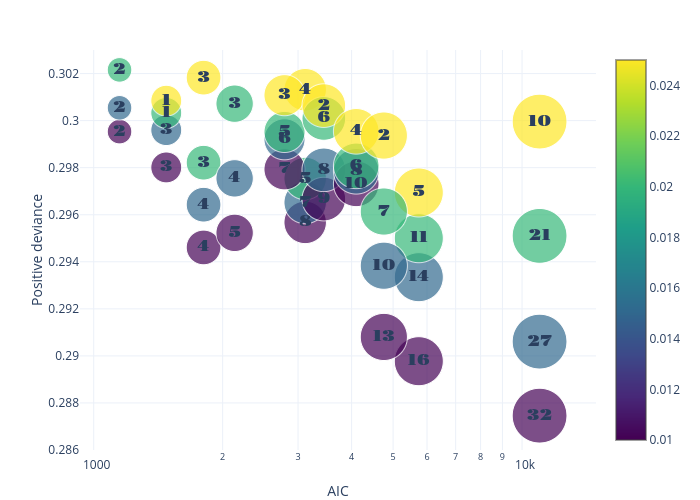
\includegraphics[scale=0.5]{gridaravo}
	\caption{Positive deviance as a function of the Akaike Information Criterion (AIC). Each point represented with a circle indicates a configuration of the hyperparameters. Circle size is proportional to embedding size. Circle color represents the value of the lasso penalty parameter $\lambda$ ranging from 0.01 (darker blueish colors) to 0.03 (brighter yellowish colors). The labels correspond to the effective dimension (non-zero components). Larger embeddings lead to a higher model complexity which explains the increasing trend in AIC values with the increase in embedding size. Higher values of $\lambda$ (yellowish points) result in fewer retained components and larger deviance scores. The combination $(\lambda=0.01,d=4)$ provides the best compromise between model complexity and performance.  \url{https://chart-studio.plot.ly/~socco/45}}
	\label{gridaravo}
\end{figure}

\subsubsection{Plant habitat suitability}
Next, we analyze the parameters and performances of the HSM fitted on plant occurrences. Results are summarized by plant genus groups in Figure \ref{hsmaravo}. The model predicts habitat suitability with at least $70\%$ AUC score for all genuses. The analysis of environmental variable importance shows the dominance of Snow duration followed by zoogenic disturbances, the site form and aspect. Physical disturbance and slope weights were neglectible, probably due to their correlation with Snow. 

\begin{figure}[bthp]
  \centering
  \inclPlt{7}{box_AlpsHSMw}
  \inclPlt{8}{scatter_AlpsPlantScores}
  \caption{Habitat Suitability Model variable importance and prediction performances per genus.}
  \label{hsmaravo}
\end{figure}

\subsubsection{Analyzing the functional meaning of plant embeddings}
Then, we investigate the functional determinants of the associations diversity. To do so, we compute the mutual information between the learnt embeddings and the plant traits (reported in \cite{choler2005consistent}). The Mutual Information \cite{shannon1949mathematical} is an unbounded symmetric and positive score that measures the amount of information contained in one random variable about another. It quantifies the reduction in uncertainty about one random variable given knowledge of another. Zero mutual information indicates independence.\\

In general, we expect traits related to dispersal capabilities (seed, spread) to impact the prevalence of the species, consequently increasing or decreasing the opportunity to affect other species (interaction probability). As a result, we expect such traits to have a higher mutual information with effect embeddings than with response embeddings. Conversely, traits related to nutrient uptake and biomass accumulation potential capture competitive or cooperative abilities of the plant species. Hence, we would expect a high mutual information between these traits and both responses and effects embeddings.\\

A histogram of the mutual information between each trait and embedding dimension is shown in Figure~\ref{mitraitemb}.  The result indicate a relatively significant contribution of the Nitrogen mass and Spread to the plants response, whereas the angle was found independent. The Specific Leaf Area contributes significantly to the effect in addition to the Nitrogen mass and on a lesser extent Spread. Height is reported as related to both parameters. \\

\begin{figure}[bthp]
  \inclPlt{9}{hist_AlpsMIEff}
  \inclPlt{10}{hist_AlpsMIRes}
	\caption{Mutual information between plant traits and their latent representations. Each bar concerns a specific trait, it represents the stack of mutual information scores from the first to the last (fourth) embedding dimension. The lower (resp. upper) figure shows the results for the response (resp. effect) embeddings.} \label{mitraitemb}
\end{figure}

\subsubsection{Plant associations on a mesotopographic gradient}
Finally, we analyze the inferred associations and the overall network topology in light of existing literature on alpine plants interactions \cite{choler2001facilitation}.\\

We perform a hierarchical clustering on both rows and columns of the association matrix to obtain effect and response groups (structural roles), which are displayed in Figure~\ref{assocplant:a}. In parallel, we apply the modularity maximization algorithm on the association network to identify densely connected modules, referred to as communities \cite{gauzens2015trophic}. After that, we map the structural roles within the modules to create the group-level network.\\

Four densely connected modules stand out. They are structured along the mesotopographical gradient. 
\begin{enumerate}
	\item High-altitude, dry and windy communities densely connected by positive associations: (i) unselective commensalism of forbs by dominant graminoids, (ii) facilitation between graminoids and tall herbs. The latter act as hubs connecting the high elevation sites to the adjacent sites. 
	\item Mid-gradient communities composed of two groups: (i) Tall herb grasslands occuring in favorables conditions, mostly structured by negative associations (ammensalism and competition); (ii) Short herb meadows, prone to zoogenic disturbance. They present higher abundances when co-occuring with tall herbs. Through their spreadth they also play a central role in connecting extreme and favorable sites' communities. 
	\item Chinopholous (cold-resistant) vegetation appearing on late-melting sites. They cohabitate positively with some short-herbs but are negatively affected by forbs and tall herbs. 
	\item North-facing isolated communities dominated by Salix Herbacea negatively associated with high-altitude communities and characterized by high eccentricity.
\end{enumerate}

Modules identified on the basis of link density by the modularity maximization algorithm are spatially structured. Hence, the network of modules reflect the spatial connectivity and as a result the turnover over the gradient. Within each community, we identify various subgroups based on different responses (incoming edges) or effects (outgoing edges) to other groups.\\

For instance, the high-elevation module (pink nodes) comprises three subgroups with different structural roles. Graminoids dominate these communities, they provide wind protection to forbs and some tall herbs (Festucal Violacea, Trifolium Alpinum). The latter also occur on grasslands where they compete with each other. Hence, this subgroup is separated from other forbs despite their cohabitation and the similar response to graminoids.\\ 

As reported in the literature (\cite{callaway2002positive},\cite{choler2005consistent}), the abiotic stressors strongly structure the distribution of the plant species and the dominant interaction types. Indeed, more positive associations are reported in stressful conditions (high-elevation and late-melting sites). Particularly, the average snow duration seems to be the major structuring force. 
     

\begin{figure}[bthp]
	\begin{subfigure}{\textwidth}
		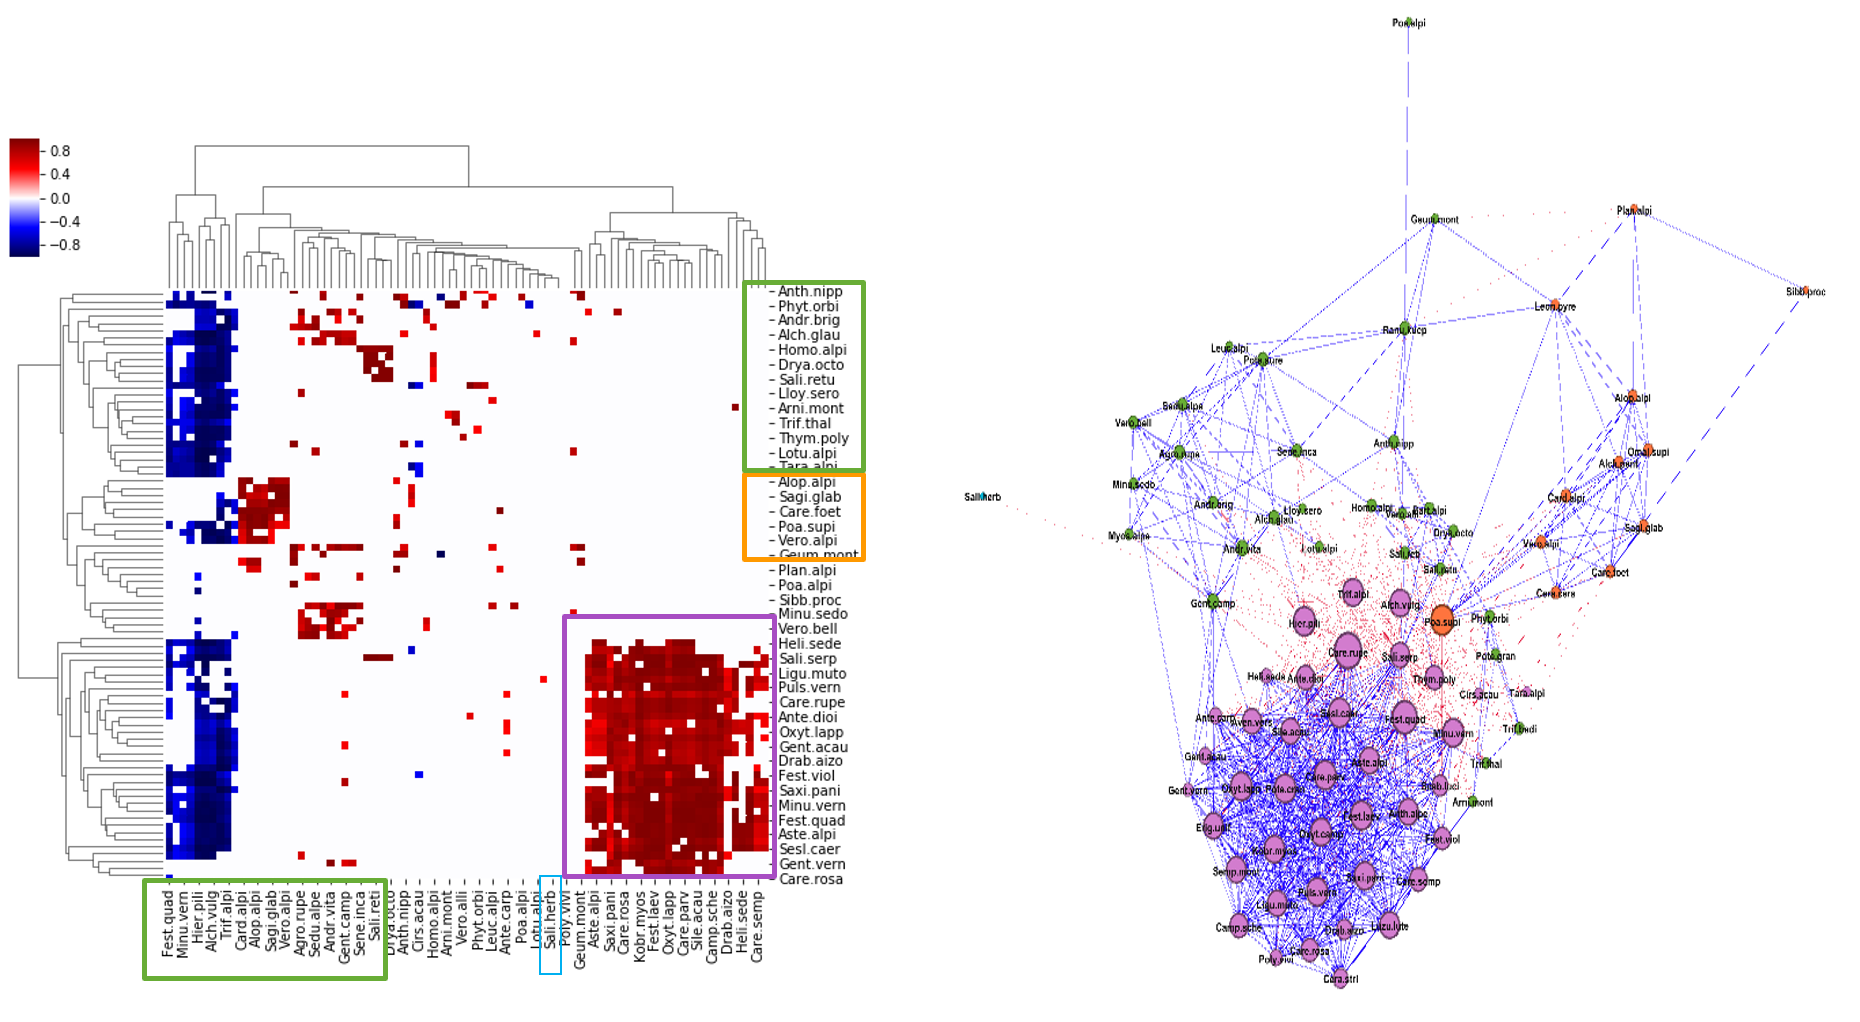
\includegraphics[scale=0.4]{aravoassoc}
		\caption{Inferred plant association network. } \label{assocplant:a}
	\end{subfigure}
	\newline
	\begin{subfigure}{\textwidth}
		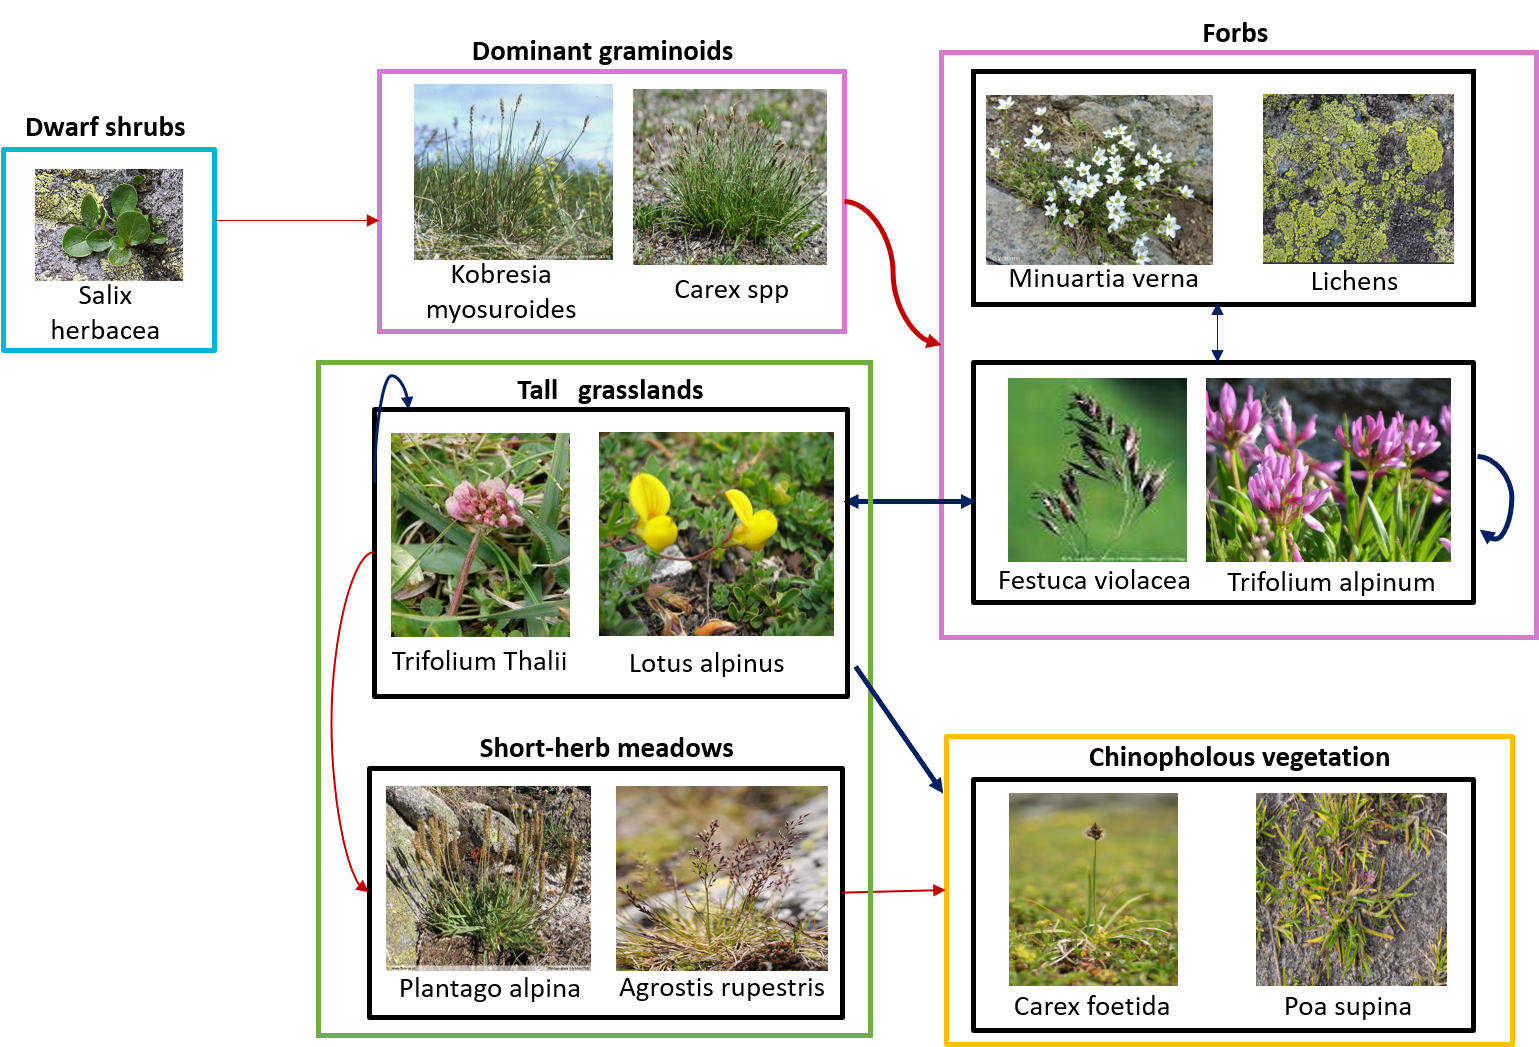
\includegraphics[scale=0.4]{groups}
		\caption{Summary network of plant associations.} \label{assocplant:b}
	\end{subfigure}
	\caption{Plant associations on an alpine mesotopographic gradient. Subfigure (a) shows the normalized pairwise associations on the left and the corresponding network on the right. Blue (resp. red) edges indicate negative (resp. positive) edge weights. Node colors on the graph represent communities identified by the modularity maximization algorithm \cite{newman2006modularity}. We highlight the communities composition using colored squares on the matrix on the right. Species in the association matrix are grouped based on a hierarchical clusterings performed rowise (yielding response groups) and columnwise (yielding effect groups). Subfigure (b) summarizes the association network at the level of previously identified groups. Edge thickness is proportional to the number of links between the interacting group pair.} \label{assocplant}
\end{figure}

\section{Discussion}
%Qu'est-ce qu'on propose ?%
We first develop a probabilistic model of multispecies abundances that accounts for habitat suitability as well as biotic associations. We parameterize this model with an asymmetric association matrix computed from two sets of low-dimensional embeddings representing: the effect present species have on others' abundance, and the response to other species' effects. We then use the model to recover meaningful associations given species abundances. \\

%Rebondir sur les résultats%
We use a process-based simulation model to generate synthetic community datasets. By analyzing the observed co-occurrence and pairwise conditional abundances, we note that co-occurrence levels can be high even on known competing pairs if the species pool is small and the communities' carrying capacity is large. On the other hand, the abundance reflects better the nature of associations as it is lower than average in presence of negative associations and higher with positive associates. Nonetheless, pairwise abundance effects may turn out to be neutral in presence of multiple confounding effects (Boulangeat et al 2012). Consequently, one should model the pairwise associations conditioned on all other species in order to isolate the different opposing influences. For instance, given a triplet A, B, C such that A (resp. C) influences B positively (resp. negatively). If the same strength is applied by A and B we may observe that all pairs are independent, unless we evaluate the association $ A -> B $ conditioned on C and $C -> B$ conditioned on A. In any case, we still need separate observations where we could quantify both associations separately. \\

Thereafter, we test the ability of the model to recover simulated associations. We find that the model is able to disentange positive, negative and neutral associations. But, it generates many spurious associations due to high levels of co-occurrence induced by the simulation model. Our model is able to recover positive associations between species with similar abiotic niches, for two reasons. First, it does not rely on residuals unexplained by the SDM. Instead, it conditions on the habitat suitability for both species hence the probability of them co-occurring would induce a potential for facilitation. Second, the association is evaluated on the basis of abundance variation in presence of the other species. \\ 

Afterwards, we apply the inference model on plants distributed along a mesotopographical gradient in the French Alps. The associations identified by the algorithm conformed to most of the important specific relationships that we expect to find in the upland plant community (\cite{choler2001facilitation}), giving us confidence in the novel methods presented here. We observe more positive associations in extreme conditions (dry, windy or frozen) and negative ones in favorable sites, confirming the stress-gradient hypothesis (\cite{callaway2002positive}). We illustrate using the results on Aravo dataset some of the possibilities allowed by the model. For instance, we can use the association matrix to populate a network, study its modular structure through community detection algorithms and analyze the structural roles, including effect and response groups, occupied by species within communities. Such information is useful to evaluate the functional redundancy within communities. Second, we argue that the learnt representations can be related to functional traits of the species, providing the appropriate traits are measured, to identify the functional drivers of network structure. \\

It is now agreed upon that inferred associations are not biological interactions. They represent significant spatial colocation or dislocation patterns, that are informative in a predictive rather than causal way (\cite{milns2010revealing}). The specific mechanism that led to these patterns may vary from pair to pair, ranging from direct interactions (e.g trophic), to indirect interactions (e.g engineering). \\

The problem of inferring associations from co-occurrence is a major part of ecological modeling publications, as much as biomedical and bioinformatics literature. Existing approaches include JSDMs (\cite{ovaskainen2017make}) which rely on explaining residual correlations by biotic effects but cannot by design model asymmetric associations. Other major state of art methods are based on probabilistic graphical models including Markov Random Fields (\cite{harris2016inferring},\cite{chiquet2018variational}) and Bayesian networks (\cite{trifonova2015spatio} \cite{aderhold2012hierarchical}). The former yields undirected networks while the latter impose a directed acyclic structure to the network of associations forbidding feedbacks and the modeling of asymmetric effects. \\

The most challenging part of this task is that it is completely unsupervised, with no prior or guidance on the expected associations or network. Hence, validating the resulting associations is tricky. It is still feasible to evaluate the veracity of the type of associations by using an edge classification scheme and a list of potential interactions as we've shown. However, it is far more difficult to validate the strength of associations especially when working with snapshot data. As many associations would have a strength around zero, it is also valuable to ask whether one should use higher thresholds to decrease the amount of spurious associations and increase model precision and how to select these thresholds ? Moreover, because many processes influence community assembly, multiple scenarios could lead to the same communities making this problem unidentifiable. In this case, we need not one expected list of associations but all the possible ones or a goodness-of-fit measure that accounts for equivalence between different association combinations. \\

A possible way to prevent the unidentifiability issue is to include known information on ecological interactions in the model \cite{cazelles2016theory}. For instance, \cite{staniczenko2017linking} use a Bayesian network with a structure defined a priori, and trains its parameters using an SDM to predict species occurrence probabilities. In our case, such constraints can be defined by altering the biotic context definition. One direct way to do it is to consider a customized biotic context for each species composed of the set of its potential interaction partners in a regional metaweb. \\

There is now growing evidence that ecological interactions are context-dependent (\cite{poisot2015beyond}, \cite{tikhonov2017using}), we show in appendix B how to infer associations whose strength is modulated by other covariates (e.g: stress, presence of predator, etc.) Recently developed models account for association variability as a function of the environmental context (Tikhonov et al 2017, Clark et al in prep). Despite the new possibilities offered by these developments, the question of how to validate their results still araises itself. \\

Finally, the model is also useful to make conditional predictions of abundances. Another possible usage is to perform link prediction on an incomplete network. The idea is to complete the associations involving a target species by leveraging information from similar node species. \\ 
 
\section{Conclusion}
Biological interactions and other processes induce spatial patterns of co-occurrence. Our objective is to disentangle these processes and isolate species dependencies. We present a model of species co-abundances as a function of the habitat and biotic associations. We propose an asymetric scheme for modeling associations that is based on learning latent representations of species responses and effects. Future efforts should be directed towards a combination of prior knowledge on the complete or partial topology of the association networks to guide the inference process. Along with that, a strong theory of how known ecological interactions influence the co-distribution of species is needed to support all these models.   

\appendix

\section{Extensions of the biotic context definition}
\label{sec:alt-bio}

\subsection{Adding conditioning covariates}
In the base model, the estimation of any pairwise interaction is oblivious to the abiotic or biotic conditions surrounding it. To account for these neighborhood conditions, we extend the base model by allowing the embeddings used to represent the biotic context to depend on some chosen variables.\\

Each site is associated to $p$ conditioning covariates, These covariates are stored alongside an offset in a $n \times (p+1)$ matrix $V$, such that each of the first $p$ columns of $V$ contains the values of the corresponding covariate for the different sites while the last column is filled with ones. 
Then, given an embedding dimension $d$, the covariates are mapped to $d$ dimensions by applying a regression with a weight matrix $W \in \mathbb{R}^{d \times (p+1)}$. The resulting conditioning vectors are such that $\condv_\site = Wv^{T}_{\site}$.\\

The extended biotic context is then written as follows, where $\odot$ is the element-wise vector product: 
\begin{equation*}
  \BioEff_{\site\spc} = \condv_{\site} \odot \big(\frac{1}{\abs{\BioCont_{\site\spc}}} \sum_{\ospc \in \BioCont_{\site\spc}} \abdv_{\site\ospc} \Resv_{\ospc} \big)
  = \frac{1}{\abs{\BioCont_{\site\spc}}} \sum_{\ospc \in \BioCont_{\site\spc}} \abdv_{\site\ospc} \cdot (\condv_{\site} \odot \Resv_{\ospc}) 
\end{equation*}

The biotic associations can be recovered as in the base model, by isolating the pairwise interactions in the response variable. However, in this case, the associations we obtain are represented by a three-dimensional tensor instead of a two-dimensional matrix. Each slice along the first dimension of this tensor represents a local association network.
\begin{align*}
  \Assv_{\site\spc\ospc} &= \sum_{l=1}^{d} (\condv_{\site} \odot \Effv_{\spc} \odot \Resv_{\ospc})_l \\
  \eta_{\site\spc} &= \linkf\big( \sum_{\ospc \in \BioCont_{\site\spc}} \abdv_{\site\spc}  \Assv_{\site\spc\ospc} + o_j\big)
\end{align*}

By incorporating the environmental covariates on the latent space, we gain two desirable properties. First, we get a fixed number of parameters that is a factor of the embedding dimension, which is significantly smaller than the number of modeled species. Second, we ensure species with similar latent traits, as captured by the response and effect embeddings, share associations regardless of the surrounding conditions. As a result, response or effect groups of species computed from the learnt embeddings remain consistent in the environmental space. 

\subsection{Temporal extension}
%Drawback of basic model, causality % 
When longitudinal data are available, we denote the abundance of species $\spc$ at site $\site$ at time-point $t$ as $\abdv_{\site\spc}^{(t)}$. Accordingly, the definition of the biotic context for a target species at a given time-point is extended to contain the species, including the target, that were observed in the previous time-point:
\begin{align*}
  \BioCont_{\site\spc}^{(t)} &= \{\ospc \in \spcS, \abdv_{\site\ospc}^{(t-1)} > 0 \} \\
  \BioEff_{\site\spc}^{(t)} &= \frac{1}{\abs{\BioCont_{\site\spc}^{(t)}}} \sum_{\ospc \in \BioCont_{\site\spc}^{(t)}} \abdv_{\site\ospc}^{(t-1)}  \Resv_{\ospc}
\end{align*}
% Graphe dynamique déroulé puis moralisé %

\subsection{Spatial extension}
Given a function $\dst$ that measures the distance between any pair of sites and a radius $r$, we consider a spatial extension of the base model where the biotic context is defined to contain species that were observed at locations within distance $r$ of the considered site.
\begin{equation*}
  \BioCont_{\site\spc} = \{(\ospc, l) \in \spcS \times \siteS, \abdv_{l\ospc} > 0 \text{ and }  \dst(\site, l) \leq r\}
\end{equation*}

One can use multiple radius values customized to the dispersal abilities of each target group or species for instance. The effect of each contextual element is weighted in inverse proportion to its distance to the target location. The hyperparameter $\tau$ controls the decrease in weight per unit of distance. Similarly, $\tau$ can be customized for each group of species based on expert knowledge.  
\begin{equation*}
  \BioEff_{\site\spc} = \sum_{(\ospc, l) \in \BioCont_{\site\spc}} \abdv_{l\ospc} \cdot \exp(-\tau \dst(\site, l))
\end{equation*}
%Substituting time for space. 
%space for time substitution, dispersal mechanisms (negative context and competition)

\subsection{Graph extension}
So far, we defined the biotic context using the community composition in terms of species, possibly involving their abundances. At this point, we are able to capture pairwise additive effects. However, we miss the impact of interactions between context species or the whole network structure around the target location on the abundance distribution of the target group, \emph{contextual network}.\\ 

Fortunately, graph embedding algorithms permit the incorporation of structured data such as knowledge graphs into predictive models. For instance, we can redefine the biotic context as the interaction network at site of interest $\site$ minus the target species $\spc$, noted $G_{\site/\spc}$. The context embedding is then obtained by applying a graph kernel function $\krnf$ with parameter $\theta$ on the contextual network

\begin{equation*}
  \BioEff_{\site\spc} = \krnf(G_{\site/\spc}; \theta)\,. 
\end{equation*}

\bibliographystyle{acm}
\bibliography{bib}	

\end{document}
